\section{Study}
\label{sec:study}

To understand how programmers use regular expressions in Python projects, we scraped \DTLfetch{data}{key}{nProjScanned}{value} Python projects from GitHub, and recorded regex usages for analysis. Throughout the rest of this paper, we  employ the following terminology:\\

\noindent \textbf{Utilization}: A \emph{utilization} occurs whenever a developer uses a regex  in a project.  We detect utilizations by recording all calls to the {\tt re} module in Python.
Within a particular file in a project, a {utilization} is composed of a function, a pattern, and 0 or more flags.  Figure~\ref{fig:exampleUsage} presents an example of one regex {utilization}, with key components labeled. The function call is {\tt re.compile}, \verb!(0|-?[1-9][0-9]*)$! is the regex string, or pattern, and {\tt re.MULTILINE} is an (optional) flag. This {utilization}  will compile a regex object in the variable {\tt r1} from the pattern \verb!(0|-?[1-9][0-9]*)$!, with the \verb!$! token matching at the end of each line because of the {\tt re.MULTILINE} flag. Thought of another way, a regular expression  utilization is one single invocation of the {\tt re} library.\\





\begin{figure}[tb]
\centering
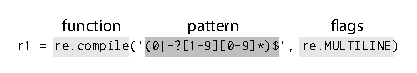
\includegraphics[width=\columnwidth]{../illustrations/exampleUsage.eps}
\caption{example of one regex utilization}
\label{fig:exampleUsage}
\end{figure}



\noindent \textbf{Pattern}: A \emph{pattern} is extracted from a utilization, as shown in Figure~\ref{fig:exampleUsage}. In essence, it is a string, but more formally it is an ordered series of regular expression language feature tokens.  The pattern in Figure~\ref{fig:exampleUsage}  will match if it finds a zero at the end of a line, or a (possibly negative) integer at the end of a line (i.e., due to the {\tt -?} sequence denoting zero or one instance of the {\tt -}).

Note that because the vast majority of regex features are shared across most general programming languages (e.g., Java, C, C\#, or Ruby), a Python {pattern} will (almost always) behave the same when used in other languages, whereas a utilization is not universal in the same way (i.e., it may not compile in other languages, even with small modifications to function and flag names).
As an example, the {\tt re.MULTILINE} flag, or similar, is present in Python, Java, and C\#, but  the Python {\tt re.DOTALL} flag is not present in C\# though it has an equivalent flag in Java.
%\todo{Carl: check the above paragraph}

In this work, we primarily focus on patterns since they are cross-cutting across languages and are the primary way of specifying the matching behavior for every utilization. Next, we describe the research questions and how the data set was collected and analyzed.

\subsection{Research Questions}
\label{sec:rqs}
To understand how regular expressions and regular expression features are used in Python projects, we aim to answer the following research questions:\\

\noindent \textbf{RQ1:} How  is the {\tt re} module used in Python projects?

We measure how often calls are made to the {\tt re} module per file and per project in Python projects.
To provide context as to the overlap among regular expression strings used in Python, we explore the most common regex {patterns} across all utlizations.\\

\noindent \textbf{RQ2:} Which regular expression language features are most commonly used in python?

We consider regex language features to be tokens that specify the matching behavior of a regex pattern, for example,  the {\tt +} in {\tt ab+}.  All studied features are listed and described in Section~\ref{study:corpus} with examples.\\

\noindent \textbf{RQ3:} What is the impact of \emph{not} supporting various regular expression features on tool users and designers?
%\textbf{RQ3:} What is the impact of \emph{not} supporting various regex features on tool designers and users?

We use semantic analysis to illustrate the impact of missing features on a tool's applicability by identifying what each feature (or group of features) is commonly used for. \\


Next, we describe how the corpus of regex patterns was built, how features were analyzed, and how the clustering was performed.
%\todo{Is this still the case?}
%Since our semantic analysis is based on Rex, this semantic analysis cannot be applied to all features studied.  For these unsupported features, we use 6 string similarity metrics (Jaro-Winkler, Levenshtein, Longest Common Substring, Sift3, Jaccard and Cosine) to build similarity matrices.  As before, these matrices are used to find clusters of regexes, which are used to interpret what a feature is used for.




\subsection{Regex Corpus}
\label{study:corpus}
%Github is a popular project hosting site containing over 100,000 Python projects.  
Using the GitHub API, we scraped \DTLfetch{data}{key}{nProjScanned}{value} Python projects that had at least one call to the {\tt re} module. \todo{how many projects were scraped but did not have a call to the {\tt re} module?}
%The GitHub API assigns an integer identifier to each repository and can be used to clone relevant repositories for analysis.  Using the \url{http://api.github.com/repositories?since=N} interface page, we launched 32 scrapers to find repositories containing Python code.  The Github interface provides information about the first 100 repository IDs since the {\tt N} value on a single results page.  Each scraper used this information to identify repositories containing Python.  When a scraper was done with one page, it continued on to the next 100 repository IDs by using the interface again with {\tt N} now equal to the last repository ID on the current page.  Using this process, each scraper paged through the next available 1,000 repositories, cloning and scanning Python projects as they were found.  Each scraper started at a different {\tt N} value, with the first scraper starting at 0.  Scraper start indices were spaced by 262,144 so as to investigate within the first 8 million repositories.  At the time scraping was performed, the highest repoID was over 32 million, so we were cloning projects in the lowest fourth of the available space of IDs.  After this process was complete, \DTLfetch{data}{key}{nProjScanned}{value} Python projects had been cloned and scanned.
%For each project, we used Astroid\footnote{\url{https://bitbucket.org/logilab/astroid}} to build the AST of each Python file and find utilizations of Python's {\tt re} module. This ensured that all utliizations of the {\tt re} module were captured for analysis.
Each project's commit history was scanned at 20 evenly-spaced commits.  If the project had fewer than 20 commits, then all commits were scanned.  The most recent commit was always included, and the spacing between all other chosen commits was determined by dividing the remaining number of commits by 19 (rounding as needed). 
All regex utilizations were obtained, sans duplicates. Within a project, a duplicate utilization was marked when two versions of the same file have the same function, pattern and flags.  In the end, we observed and recorded \DTLfetch{data}{key}{nUsages}{value} non-duplicate regex utilizations in \DTLfetch{data}{key}{nProjScanned}{value} projects.

In collecting the set of distinct patterns for analysis,  we ignore the \DTLfetch{data}{key}{percentBadFlags}{value}\%  of utilizations using flags, which can alter regex behavior.  An additional \DTLfetch{data}{key}{percentInvalidPattern}{value}\% of utilizations contained patterns that could not be compiled because the pattern was non-static (e.g., used some runtime variable), or because of other unknown parsing failures.

The remaining \DTLfetch{data}{key}{percentCleanUsages}{value}\% (\DTLfetch{data}{key}{nCleanUsages}{value}) utilizations were collapsed into \DTLfetch{data}{key}{nDistinctPatterns}{value} distinct pattern strings using sql.  Each of the pattern strings was pre-processed by removing Python quotes (\verb!`\\W!' becomes \verb!\\W!), unescaping escaped characters (\verb!\\W! becomes \verb!\W!) and parsing the resulting  string using an ANTLR-based, open source PCRE parser\footnote{\url{https://github.com/bkiers/pcre-parser}}.

This parser was unable to support \DTLfetch{data}{key}{percentUnicode}{value}\% (\DTLfetch{data}{key}{N_UNICODE}{value}) of the patterns due to unsupported unicode characters.  Another \DTLfetch{data}{key}{percentAlien}{value}\% (\DTLfetch{data}{key}{N_ALIEN}{value}) of the patterns used regex features that we have chosen to exclude in this study because they did not appear often enough (e.g., Reference Conditions).  The \DTLfetch{data}{key}{nCorpus}{value} distinct pattern strings that remain were each assigned a weight value equal to the number of distinct projects the pattern appeared in.  We  refer to this set of weighted, distinct pattern strings as the \emph{corpus}.

\subsection{Analyzing Features}
\label{study:features}
For each escaped pattern, the PCRE-parser produces a tree of feature tokens, which is converted to a vector by counting the number of each token present in the tree.  For a simple example, consider the patterns in Figure~\ref{fig:featureParsing}.  The pattern \verb!`^m+(f(z)*)+'! contains four different types of tokens. It contains the kleene star (KLE), which is specified using the asterisk \verb!`*'! character, additional repetition (ADD), which is specified using the plus \verb!`+'! character, capture groups (CG), which are specified using pairs of parenthesis \verb!`(...)'! characters, and the start anchor (STR), which is specified using the caret \verb!`^'! character at the beginning of a pattern.

\begin{figure}[tb]
\centering
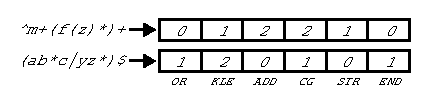
\includegraphics[height=0.6in]{../illustrations/featureParsing.eps}
\caption{Two Patterns Parsed into Feature Vectors}
\label{fig:featureParsing}
\end{figure}

Once all patterns were transformed into vectors, we examined each feature independently for all patterns, tracking the number of patterns it was in, and the size of the sets of projects and files that the patterns containing the features appeared in at least once.
%Our semantic analysis is dependent on the use of Rex to generate strings so we can identify semantically related clusters. For three common features unsupported by Rex, we rely on syntactic analysis to determine similarity among regular expressions containing those features. For those features supported by Rex, we cluster the regular expressions based on semantic diversity.

\subsection{Clustering and Semantic Analysis}
Our semantic analysis clusters regular expressions by their behavioral similarity. 
Consider two unspecified patterns {\tt A} and {\tt B}, a set {\tt mA} of 100 strings that pattern {\tt A} matches, and a set {\tt mB} of 100 strings that pattern {\tt B} matches.  
If pattern {\tt B} matches 90 of the 100 strings in the set {\tt mA}, then {\tt B} is 90\% similar to {\tt A}.  
If pattern {\tt A} only matches 50 of the strings in {\tt mB}, then {\tt A} is 50\% similar to {\tt B}.  
We use similarity scores to create a similarity matrix as shown in Figure~\ref{fig:minimalMatrix}.  
In row {\tt A}, column {\tt B} we see that {\tt B} is 90\% similar to {\tt A}.  
In row {\tt B}, column {\tt A}, we see that {\tt A} is 50\% similar to {\tt B}.  Each pattern is always 100\% similar to itself, by definition. 


\begin{figure}[tb]
\centering
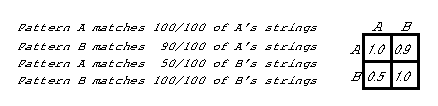
\includegraphics[height=0.6in]{../illustrations/minimalMatrix.eps}
\caption{A Similarity Matrix Created by Counting Strings Matched}
\label{fig:minimalMatrix}
\end{figure}


In the implementation, strings are generated for each pattern using Rex~\cite{rex}. 
\todo{explain how Rex generated strings. How likely is Rex to enumerate the same regular expressions for similar
regular expressions?}
Our goal is to generate 384 strings for each pattern to balance the runtime of the similarity analysis with the precision of the similarity calculations. 
 Since Rex does not support all the features present in the corpus, we could only generate sets of matching strings for 9,727 (70\%) of the \DTLfetch{data}{key}{nCorpus}{value} patterns in the corpus. The impact is that 270 projects were excluded from the data set for the similarity analysis. Omitted features are indicated in Table~\ref{table:featureStats}, as described in Section~\ref{results:rq3}. 
The generated strings for each pattern are used to measure the pairwise similarity for all patterns and construct the similarity matrix. 
%If Rex rejects the pattern, or fewer than 384 strings are generated, we do not include that pattern in the similarity analysis.
%The average number of generated strings per pattern was \todo{X} with a standard deviation of \todo{Y}. The maximum number generated was \todo{Z-these3:programming project for later tonight}.
%At least one pattern from the 9727 patterns that Rex was able to generate matching strings for can be found in 1375 of the 1645 projects containing at least one utilization.  

Once the similarity matrix is built, the values of cells reflected across the diagonal of the matrix were averaged to create a half-matrix of undirected similarity edges, as illustrated in Figure~\ref{fig:matrixToGraph} \todo{remove the text file from the figure}. This facilitated clustering by means of the  Markov Clustering (MCL) algorithm\footnote{\url{http://micans.org/mcl/}}.  
We chose the mcl clustering tool because it offers a fast and tunable way to cluster items by similarity and it is particularly useful when the number of clusters is not known \emph{a priori}.
We note that Markov clustering can be tuned using many parameters, including inflation and filtering out all but the top-k edges for each node.  After exploring the quality of the clusters using various tuning parameter combinations, the best clusters (by inspection) were found using an inflation value of 1.8 and k=83.
The end result is clusters of highly semantically similar regular expressions. 



%Using all similarity values in this half-matrix above 0.75, we created a text file specifying the edges of a graph.  This process is illustrated in Figure~\ref{fig:matrixToGraph}.
%The first matrix represents all pairwise similarity values between the four regexes: A, B, C, and D.  The second matrix represents the average of cells reflected across the diagonal of the matrix.  For example the value of row A, column C (0.9) represents the similarity of C to strings generated by Rex for regex A.  The value of row C column A (0.6) represents the similarity of A to strings generated by Rex for regex C.  The average of the two values is 0.75, which goes into row C, column A in the half-matrix.  For every value of 0.75 or greater, an edge is written to \emph{out.abc}.
%Note that pairs DB and DC are omitted from the final file because their similarities are lower than the threshold.  The \emph{out.abc} generated file  is fed as input to the Markov Clustering Algorithm, and the top 100 clusters were catagorized by inspection into six categories of behavior (see Section~\ref{results:rq3}).
%
%Once the similarity matrix is built, clusters of regexes with similar behavior are discovered using Markov Clustering\footnote{\url{http://micans.org/mcl/}}.  
%We chose the mcl clustering tool because it offers a fast and tunable way to cluster items by similarity and it is particularly useful when the number of clusters is not known \emph{a priori}.


%We are interested in what behaviors users are trying to get when using regexes, and we know that the exact same behavior, or very similar behavior can be specified in many ways.  For example, the three patterns \verb!`\W'!, \verb!`[^\w]'!, \verb!`[^a-zA-Z0-9_]'! all specify the same matching behavior.  Even if we create a slightly different pattern that matches one more character, for example \verb!`[\W_]'!, most strings that match the first three equivalent patterns will also match the different pattern.


%As explained in Section~\ref{sec:rqs}, we used these sets of matching strings to  measure the pairwise similarity between regular expressions and create a behavioral similarity matrix.  We will refer to a cell of this matrix with row index {\tt i} and column index {\tt j} as {\tt M[i][j]}.  For each pattern at index {\tt i}, we used Rex to create a set of matching strings which we will refer to as {\tt matching\_strings\_i}.  Then for every pattern at index {\tt j}, we set the value of {\tt M[i][j]} equal to the fraction of strings in {\tt matching\_strings\_i} that the pattern at index {\tt j} matched.




\begin{figure}[tb]
\centering
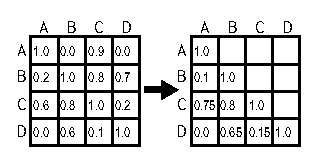
\includegraphics[width=\columnwidth]{../illustrations/matrixToGraph.eps}
\caption{Creating A Similarity Graph From A Similarity Matrix}
\label{fig:matrixToGraph}
\end{figure}



\todo{Carl - can you fix this before the ICSE deadline?}
We note that there was an operational error in pulling patterns from our database prior to the similarity analysis and clustering, so that 224 patterns (2.3\%) of the 9,727 patterns were omitted. These were duplicate patterns that were quoted differently (for example \verb!`\W'! and \verb!"\W"!).  The result of this error is a slight underestimate in number of projects per pattern (and per cluster), and a slight over-estimate in the pattern, file and project statistics shown in Table~\ref{table:featureStats}.  We do not believe that this error affects our conclusions.


%Most patterns do not belong in a cluster (for example a very specific pattern like \verb!<title>[^<]*Revision \d+:!), so after clustering is done only 2727 patterns are included, and only 999 projects have any of these patterns in them.

